%  \documentclass[DIV=12, a4]{scrartcl}
%\documentclass[12pt, a5]{scrartcl}

% \documentclass[a4paper]{report}
% \usepackage[
% % fancytheorems, 
% noindent, 
% %spacingfix, 
% %noheader
% ]{vanilla}


\documentclass[a4paper]{scrreprt}
\usepackage[
fancytheorems, 
noindent, 
% %spacingfix, 
% %noheader,
fancyproofs
]{adam} 

\usepackage{tikz}

% \usepackage{subfig}

\setcounter{chapter}{-1}

\title{Numbers and Sets}
% \subtitle{Adam Kelly}
\author{Adam Kelly}
% \date{Michaelmas 2020}
\date{\today}

\begin{document}

\maketitle

\begin{abstract}
	
	% \vspace{2\baselineskip}
	% {\color{red} None of the notes here have been reviewed at all, and are just exactly what was taken down live in the lectures. I would turn around now and come back in a few days, when I have gone back, cleaned things up, fixed explanations and added some structure.}
	% \vspace{5\baselineskip}

	This set of notes is a work-in-progress account of the course `Numbers and Sets', originally lectured by Professor Imre Leader in Michaelmas 2020 at Cambridge. These notes are not a transcription of the lectures, but they do roughly follow what was lectured (in content and in structure).

	These notes are my own view of what was taught, and should be somewhat of a superset of what was actually taught. I frequently provide different explanations, proofs, examples, and so on in areas where I feel they are helpful. Because of this, this work is likely to contain errors, which you may assume are my own. If you spot any or have any other feedback, I can be contacted at \href{mailto:ak2316@cam.ac.uk}{ak2316@cam.ac.uk}.


	% {\color{red} Notes written upto lecture 6.}
	% During the creation of this document, I consulted a number of other books and resources. All of these are listed in the bibliography. 

\end{abstract}

\tableofcontents

\clearpage
\chapter{Introduction}

Numbers and sets is one of the first course in pure mathematics that you will take
as an undergraduate at Cambridge. In a sense, it is the `starting course', in that it will introduce you to the `pure maths' way of thinking about things. 
This introduction will happen through the lense of thinking about objects, beginning with the natural and real numbers. You will be introduced to the `thoughtful way' of thinking about such objects, that you can carry through to almost every other course in pure mathematics.

\section{Structure of the Course}

This course is divided into four sections.

\begin{enumerate}
	\item \emph{Elementary Number Theory}
	
	This is a section that almost everybody enjoys. 
	We deal with number theory first, which is elementary not in the sense that it is easy but in the sense that it is our `first steps' in the subject. The main aim of this section is to get used to the additive and multiplicative structure of the natural numbers.

	It is like that some of you will be familiar with this material already, but nothing in this section will be assumed, and everything will be built from the ground up.

	\item \emph{The Reals}
	
	This section has a different perspective, centering on the questions of \emph{what is a real number} and \emph{what can we assume about them?} This is one of the harder parts of this course, and many of the definitions contain a subtlety that is not present in other sections. 

	\item \emph{Sets and Functions}
	
	This is a `terminology' section. There is no exciting theorems, mostly notation, definitions, and so on. It is a short section, but it is somewhat boring in that sense.

	\item \emph{Countability}
	
	This section is best described as `fun with infinite sets'. It is to do with the concepts introduced in section 3 (in the sense that we are thinking about sets and functions), but it has a very different flavour. You will find results in this section that are both interesting and surprising. Almost everyone likes this section.
\end{enumerate}

Everything in the sections above makes up the `course'. If you are wondering what is examinable, it will be everything that was lectured. It is possible that this set of `lecture notes' will contain additional content that was both not in lectures and not examinable. If you want to be sure whether something you are reading here or elsewhere is examinable, you can get a more formal answer in \href{https://www.maths.cam.ac.uk/undergrad/files/schedules.pdf}{the schedules}.

\section{Books}

As with most mathematics courses in Cambridge, you will not need a textbook to follow this course. What is covered in lectures is enough to do both the example sheets and the examinations for this course. Still, you might find that a textbook can provide a different perspective, additional worked examples, and additional material that you may find informative, helpful or fun.

In particular, the following books are quite relevant/good, but there is no expectation that you will look at these.

\begin{itemize}
	\item R. T. Allenby, \emph{Numbers and Proofs}.
	
	This book is readable, easy to understand and clear.

	\item A. G. Hamilton, \emph{Numbers, Sets and Axioms}.
	
	Another readable and clear book, but with a different flavour to the previous book.

	\item H. Davenport, \emph{The Higher Arithmetic}.

	This book can be thought of as showing `where things go next'. It is very interesting, and goes quite a bit beyond this course. It is worth noting however that this book contains no exercises.
\end{itemize}

You should be able to find all of these books in either your college library or the university library.

\section{Example Sheets}

As is normal for a 24 lecture course, there will be 4 example sheets. You should be able to have a good go at the first one after lecture 3 or 4.

\section{A Brief Note About These Notes}

This set of notes differs from what was lectured in a number of areas. I have attempted to briefly outline these changes below.

In the original lecture course, there was two lectures that (informally) introduced the idea of a proof, along with examples and non-examples of what a proof is. This material has been purposefully excluded, and familiarity with proofs (and common logical notation such as $\forall$, $\exists$, and $\implies$) is assumed. 
If you are interested in reading a brief introduction to proofs, I will direct you to this \href{https://math.berkeley.edu/~hutching/teach/proofs.pdf}{quite readable introduction}.

I have also included additional exposition on the Peano axioms, along with a more detailed look at how addition, multiplication, etc are defined. In the original lectures, this material was purposefully omitted. The exposition included in these notes closely follows the development in Tao's \emph{Analysis I} (see the bibliography).

\clearpage


\chapter{Elementary Number Theory}\label{ch:1}

Number theory is the branch of mathematics that studies the properties of \emph{numbers}, with a particular emphasis on the natural numbers $\N$, the integers $\Z$ and occasionally the rationals $\Q$. In this section, we will study some of the \emph{additive} and \emph{multiplicative} structure of the integers, looking at divisors, primes and tools such as modular arithmetic. 

One of the aims of this course (and this section in particular) is to study numbers `from the ground up', being quite careful about what we assume. This goal immediately presents us with a question: what exactly is a `number'?


\section{The Peano Axioms}

What are the natural numbers? Intuitively, we might say that they are a set\footnote{We will look at sets later in the course, but an informal familiarity will be assumed from the beginning} $\N = \{1, 2, 3, \dots\}$, created by starting at $1$ and counting forward indefinitely, each time obtaining an object distinct from all of the previous ones.
	This does answer our question (a natural number is any element of $\N$), but has created a series of other questions. For example, what does it mean to `count forward', and how can it be done `indefinitely'? How are we allowed to use these natural numbers, in regard to defining things like addition and multiplication? 
	
Instead of attempting to answer these questions using our informal, intuitive definition of the natural numbers, we will instead use a definition that is more precise. Namely, we will define the natural numbers using the Peano axioms. We will state the rules or \emph{axioms} that natural numbers satisfy, which will define the natural numbers in terms of \emph{how they work}, rather than \emph{what they are}. After clearly setting out this definition, we will be in a much stronger position to write concrete mathematical proofs about the natural numbers.

\begin{definition}[Peano Axioms]
	The \vocab{natural numbers} are a set $\N$, along with a function $S: \N \rightarrow \N$ and an object `$1$' satisfying the following axioms:
	\begin{enumerate}
		\item $1 \in \N$.
		\item If $n \in \N$, then $S(n) \in \N$.
		\item $S(n) \neq 1$ for every $n \in \N$.
		\item If $n, m \in \N$ and $n \neq m$, then $S(n) \neq S(m)$.
		\item \emph{Induction}. Let $P(n)$ be any property about a natural number $n$. Suppose that $P(0)$ is true, and suppose that whenever $P(n)$ is true, $P(S(n))$ is also true. Then $P(n)$ is true for every natural number $n$.
	\end{enumerate}
\end{definition}

This should match with our original, informal definition of the natural numbers. We have formalized the `counting forward' process with the \emph{successor function} $S(n)$.

\begin{remark}
	We are going to assume various things about the way we write down natural numbers using the decimal system. You can assume that when we write something like $n = 3$, we really mean $n = S(S(1))$ etc.
\end{remark}


\subsection{Addition}

Now we have defined natural numbers, but as of yet we can do nothing more look upon them fondly and increment them using the function $S(n)$. We will now begin to remedy that by defining addition and multiplication.

\begin{definition}[Addition]
	We define \vocab{addition} to be an operation $+$ such that for $m, n \in \N$, we have $m + 1 = S(m)$, and $m + (n + 1) = (m + n) + 1$.
\end{definition}

This definition defines addition for all natural numbers by induction. We are now able to state and prove various properties of addition.

\begin{proposition}[Properties of Addition]
	For all $a, b, c \in \N$. Then
	\begin{enumerate}[label=(\roman*)]
		\item \emph{Addition is commutative}. $a + b = b + a$.
		\item \emph{Addition is associative}. $(a + b) + c = a + (b + c)$. 
		\item \emph{Cancellation law}. If $a + b = a + c$ then $b = c$.
	\end{enumerate}
\end{proposition}
\begin{proof}[Proof Sketch]
	Use induction.\footnote{The proofs for these sorts of statements tend do be slightly dull and laborious, and for this reason they have been excluded. If you wish to read them, I encourage you to consult a textbook/some other reference material.}
\end{proof}

\subsection{Order}

We can now use addition to define an ordering on the natural numbers.

\begin{definition}[Ordering of the Natural Numbers]
	Let $n, m \in \N$. We say that $n$ is \vocab{greater than or equal to} $m$, written $n \geq m$ if and only if $n = m$ or $n = m + a$ for some $a \in \N$. We say $n$ is \vocab{strictly greater than} $m$ if $n \geq m$ and $n \neq m$.
\end{definition}

\begin{proposition}[Properties of Ordering]
	Let $a, b, c \in \N$. Then
	\begin{enumerate}[label=(\roman*)]
		\item \emph{Order is reflective}. $a \geq a$.
		\item \emph{Order is transitive}. If $a \geq b$ and $b \geq c$, then $a \geq c$.
		\item \emph{Order is anti-symmetric}. If $a \geq b$ and $b \geq a$, then $a = b$.
		\item \emph{Addition preserves order}. $a \geq b$ if and only if $a + c \geq b + c$.
		\item $a > b$ if and only if $a \geq b + 1$.
	\end{enumerate}
\end{proposition}

\begin{proposition}[Trichotomy]
	Let $a$ and $b$ be natural umbers. Then exactly one of the following is true: $a < b$, $a = b$ or $a > b$.
\end{proposition}

\subsection{Multiplication}

We can also define another familiar operation, multiplication, in the same inductive/recursive fashion that we defined addition.

\begin{definition}[Multiplication]
	We define \vocab{multiplication} to be an operation $\times$ such that for $m, n \in \N$, $m \times 1 = m$, and $m \times (n + 1) = (m \times n) + m$.
\end{definition}
As before, induction implies that this is defined for all natural numbers. It also guarantees that multiplying two natural numbers is a natural number.

\begin{notation}
We will use $a \times b = a\cdot b = ab$ when referring to multiplication.
\end{notation}

\begin{proposition}[Properties of Multiplication]
	For all $a, b, c \in \N$. Then
	\begin{enumerate}[label=(\roman*)]
		\item \emph{Multiplication is commutative}. $a \times b = b \times a$.
		\item \emph{Multiplication is associative}. $(a \times b) \times c = a \times (b \times c)$.
		\item \emph{Distributive law}. $a \times(b + c) = a \times b + a \times c$. 
		\item \emph{Cancellation law}. If $a\times b = a\times c$ then $b = c$.
		\item \emph{Multiplication preserves order}. If $a < b$, then $a\times c < b \times c$.
	\end{enumerate}
\end{proposition}
\begin{remark}
	The final two statements in the proposition above, the cancellation law and that multiplication preserves order, only hold because we are dealing with natural numbers. These properties do not hold in general if we allow $a, b$ or $c$ to be integers.
\end{remark}

We could go further and define other common operations such as exponentiation, factorials and so on, all of which can be defined in the same fashion. However, in the interest of space, these definitions have been omitted.

\section{Strong Induction}

There is a more useful form of induction that can be used, now that we have defined an ordering on the natural numbers.

\begin{proposition}[Strong Induction]
	Suppose that we have some property $P(n)$ about a natural number $n$. If we have $P(1)$, and for all $n \in \N$ we have that $P(m)$ for $m \leq n$ implies $P(n + 1)$, then $P(n)$ holds for all $n \in \N$.
\end{proposition}
\begin{proof}
	This follows from ordinary induction using the property ``$P(n)$ for all $m \leq n$''.
\end{proof}

Informally, the principle of strong induction means that whenever we are proving some property $P(n)$ holds for all $n \in \N$ by induction, we can feel free to assume that $P(m)$ holds for $m \in \N$ with $m < n$.

\begin{remark}[For Pedants]
	Technically, we don't need to check the case $P(1)$ separately, as it is implied by the condition if suitably interpreted. Still, it's safer to just check $P(1)$.
\end{remark}


Some other equivalent but useful\footnote{Some texts will claim that we can replace the induction axiom in Peano axioms with one of these other forms. This is incorrect, and typically one will need to add additional axioms alongside to keep the set of axioms equivalent.} forms of induction are listed below. Let $P(n)$ be a property, then
\begin{itemize}
	\item \emph{Existence of a Minimal Counterexample}
	
	If $P(n)$ is false for some $n \in \N$, then there exists $n_0 \in \N$ such that $P(n_0)$ is false but $P(m)$ is true for all $m < n$.

	\item \emph{The Well-Ordering Principle}
	
	If $P(n)$ is true for some $n \in \N$, then there exists a minimal $n_0$ such that $P(n_0)$ is true.
\end{itemize}

\section{The Integers and Rationals}

The previous section defined the natural numbers, along with some ways that we can use them. We will now go one step further and define the \emph{integers}, and the \emph{rationals}.

\begin{definition}[Integers]
	The \vocab{integers} are a set $\Z$ consisting of all symbols $n$, $-n$ and 0, where $n \in \N$. 
\end{definition}

We can then define addition, multiplication and subtraction in (and subtraction) on the integers by extending our definition on the natural numbers in the obvious way. We can also check that the properties of addition we had before still hold. There are some additional properties that the integers have.

\begin{proposition}[Algebraic Properties of the Integers]
	Let $a, b \in \Z$. Then\footnote{These properties imply that the integers are a \emph{group}.}
	\begin{enumerate}[label=(\roman*)]
		\item \emph{Identity}. $a + 0 = a$.
		\item \emph{Existence of an Additive Inverse}. For all $a \in \Z$, there exists $b \in \Z$ such that $a + b = 0$.
	\end{enumerate}
\end{proposition}
\begin{proof}
	$a + 0 = a$ holds automatically due to our definition of addition on the integers. Then, we always have a $b \in \Z$ such that $a + b = 0$, as we can let $b = -a$.
\end{proof}

We also obtain another interesting property of multiplication.

\begin{proposition}[Zero Product Law]
	Let $a$ and $b$ be integers such that $a \times b = 0$. Then either $a = 0$, $b = 0$ or both.
\end{proposition}
\begin{proof}
	Assume for the purposes of contradiction that both $a \neq 0$ and $b \neq 0$. Then we must have either $a > 0$ or $a < 0$ by trichotomy. If $a > 0$, then $a \times b > 0$ if $b > 0$, or $a \times b < 0$ if $b < 0$. Otherwise, if $a < 0$, then $a \times b < 0$ if $b > 0$, or $a \times b > 0$ if $b < 0$. These are all possible cases, and thus we never have that $a \times b = 0$. Thus at least one of $a$ and $b$ must be zero. 
\end{proof}

\begin{remark}[Caveats]
	We noted earlier that there was some properties of the natural numbers that don't hold over the integers. Specifically, if we have $a < b$ for $a, b \in \Z$, and we multiply by a negative number, then the order is no longer preserved (it is switched). Also, the cancellation law only applies when we are cancelling a non-zero integer.
\end{remark}

We can now use the integers to define the \emph{rationals}.

\begin{definition}[Rationals]
	The \vocab{rationals} are a set $\Q$ of expressions $a/b$ for some $a, b \in \Z$, with $b \neq 0$. We will define equality between rationals such that $a/b = c/d \iff ad = bc$. 
\end{definition}

This definition implicitly defines $\Q$ using \emph{equivalence classes}, which will be discussed later. 
We need to be slightly more careful in defining addition on $\Q$, as we will need to ensure that it respects the equality relation between rationals. 

\begin{definition}[Addition on $\Q$]
	For $a/b$ and $c/d \in \Q$, we define addition such that
	$$
	\frac{a}{b} + \frac{c}{d} = \frac{ad + bc}{bd}.
	$$
\end{definition}

We will now need to explicitly check that this definition is valid.
\begin{proposition}
	Addition is well defined on $\Q$.
\end{proposition}
\begin{proof}
	Let $a/b = a'/b'$ and $c/d = c'/d'$ be rationals. We show that
\begin{align*}
	\frac{a}{b} + \frac{c}{d} &= \frac{a'}{b'} + \frac{c'}{d'} \\
\iff \frac{ad + bc}{bd} &= \frac{a'd' + b'c'}{b'd'} \\
\iff (ad + bc)(b'd') &= (a'd' + b'c')(bd) \\
\iff (ab')dd' + (cd')bb' &= (a'b)d'd + (c'd)bb', 
\end{align*}
which follows from $ab' = a'b$ and $cd' = c'd$.
\end{proof}

To see why such a check was needed, consider the following example.

\begin{example}
	We \emph{cannot} define an operation on $\mathbb{Q}$ sending $a/b \rightarrow a^2 / b^3$, as we would have $1/2 \rightarrow 1/8$ and $2/4 \rightarrow 4/64 = 1/16$, which is inconsistent.
\end{example}

We can then define multiplication in the same way as it was defined for integers, and we can check that all of the usual properties still hold. We can also define ordering, where $a/b < c/d$ if $ab < bc$. The rules from ordering $\Z$ still hold.

With all of these definitions in place, we can now start looking at some of the more interesting properties of numbers.

\section{Primes and Divisibility}

We will now begin to discuss some actual number theory, beginning with the incredibly important concept of \emph{divisibility}. You are likely to be familiar with this already, so we will jump into some definitions.

\begin{definition}[Divisibility]
	For $a, b \in \N$, we say that $a$ \vocab{divides} $b$, written $a \mid b$ if there exists some $c \in \N$ such that $b = ac$.
\end{definition}

If this is the case, we say that $b$ is a \vocab{multiple} of $a$, and that $a$ is a \vocab{divisor} of $b$. We can now define one of the most fundamental objects in number theory, the \emph{primes}.

\begin{definition}[Primes]
	A natural number $n \geq 2$ is a \vocab{prime} if its only divisors are $1$ and $n$. If a natural number is not prime, then it is \vocab{composite}.
\end{definition}

With this definition, we can begin to state and prove some interesting results about the primes, which should hint at their importance in number theory.

\begin{theorem}\label{thm:product-primes}
	Every natural number is expressible as a product of primes.
\end{theorem}
\begin{proof}
	We use induction on $n$. For $n = 2$ this is true, as $2$ is prime. Now given $n > 2$, if $n$ is prime, then we are done. If not, then $n$ is composite so $n = ab$ for some $1 < a, b < n$. By our induction hypothesis, we have $a = p_1 p_2 \cdots p_k$ and $b = q_1 q_2 \cdots q_l$ for some (not necessarily distinct) primes $p_1, \cdots p_k, q_1, \cdots, q_l$, hence $ab = p_1 \cdots p_k q_1 \cdots q_l$, which is the product of primes. Thus we are done by induction.
\end{proof}

A nice consequence of this theorem is that the primes go on forever.

\begin{theorem}[Euclid]
	There are infinitely many primes.
\end{theorem}
\begin{proof}
	Suppose there was finitely many primes, say $p_1, \cdots, p_k$. Then consider the number $N = p_1 p_2 \cdots p_k + 1$. Then $N$ has no prime factors, contradicting the fact that $n$ can be written as the product of primes\footnote{This theorem has an amusingly large number of proofs. A short discussion can be found in the book `Proofs from the Book'.}.
\end{proof}

\begin{remark}
	There is no `pattern' to the primes, in the sense that there is no algebraic formula for the $n$th prime. 
\end{remark}

So we know that a number can be written as the product of primes, but is this unique (up to some reordering)? This would seem to be true from experience, so why can't we write a number as the product of primes in two ways. For example, why can't we have $41 \times 101 = 67 \times 73$? Informally, we might think that this is impossible because we can't have 41 dividing `a bit of' 67 and `a bit of 73'. What we really need to show that prime factorization is unique is the following: For a prime $p$, if $p \mid ab$ then $p \mid a$ or $p \mid b$.

Now should this lemma be easy to prove, or hard to prove? That is, should this follow straight from definitions, or not? The answer is that it \emph{cannot} follow straight from definitions. This is because it's about `primes dividing things', but we define the primes with `things diving it'. This is the wrong way round! It will take some amount of work to be able to prove this.

\subsection{Greatest Common Divisors}

This section will begin to build some machinery that will allow us to tackle the problem of showing that prime factorizations are unique. We will begin by defining the notion of \emph{greatest common divisor}, also known as \emph{highest common factor}\footnote{This was the term used in the lectures, but I prefer greatest common divisor, so I will use that instead.}.

\begin{definition}[Greatest Common Divisor]
	For $a, b \in \N$, a natural number $d$ is the \vocab{greatest common divisor} of $a$ and $b$, written $d = \gcd(a, b)$ if
	\begin{enumerate}[label=(\roman*)]
		\item $d \mid a$ and $d \mid b$;
		\item If $c \mid a$ and $c \mid b$, then $c \mid d$.§
	\end{enumerate}
\end{definition}

We want to show that the greatest common divisor always exists.

\begin{proposition}[Divison Algorithm]
	For $n, k \in \N$, we can write $n = qk + r$, where $q, r \in \N$ and $0 \leq r < k$.
\end{proposition}
\begin{proof}
	We use induction on $N$. For $n = 1$, this is clearly true. Otherwise, given $n > 1$, we can write $n - 1 = qk + r$ by our inductive hypothesis. Then, if $r < k - 1$, we can write $n = qk + (r + 1)$, and if $r = k - 1$, we can write $n = q(k + 1)$.
\end{proof}

The division algorithm is related to the greatest common divisor using the following lemma.

\begin{lemma}[Euclid]\label{lemma:euc}
	For $a, b \in \N$, we can write $a = bq + r$ using the division algorithm. Then $\gcd(a, b) = \gcd(b, r)$.
\end{lemma}
\begin{proof}
	If $d \mid a$ and $d \mid b$, then $d \mid a - bq = r$.
	Otherwise, if $d \mid b$ and $d \mid r$, then $d \mid bq + r = a$, hence the set of common divisors between $a$ and $b$ is the same as the set of divisors between $b$ and $r$. Thus $\gcd(a, b) = \gcd(b, r)$.
\end{proof}

\begin{theorem}[Euclidean Algorithm]
	For $a, b \in \N$, if we repeatedly apply the division algorithm to get
	\begin{align*}
		a &= q_1 b + r_1 \\
		b &= q_2 r_1 + r_2 \\
		r_1 &= q_3 r_2 + r_3 \\
		&\vdots \\
		r_{n - 2} = q_n r_{n - 1},
	\end{align*}
	then $\gcd(a, b) = r_{n - 1}$.
\end{theorem}
\begin{proof}
	We repeatedly apply \autoref{lemma:euc} until we have $\gcd(a, b) = \gcd(r_{n - 1}, 0) = r_{n - 1}$.
\end{proof}

The Euclidean Algorithm gives us both a proof that $\gcd(a, b)$ exists for any natural numbers $a$ and $b$, and it also gives us an efficient way to find it.

\begin{example}
	To find $\gcd(87, 52)$, we perform the following series of steps.
	\begin{align*}
		87 &= 1 \times 52 + 35 \\
		52 &= 1 \times 35 + 17 \\
		35 &= 2 \times 17 + 1\\
		17 &= 17 \times 1,
	\end{align*}
	thus $\gcd(87, 52) = 1$.
\end{example}

\begin{notation}
	We will sometimes write $\gcd(87, 52) = \hcf(87, 52) = (87, 52) = 1$. And when $\gcd(a, b) = 1$, we say that $a$ and $b$ are \vocab{coprime} or \vocab{relatively prime}.
\end{notation}

The example above showed that $\gcd(87, 52) = 1$, so is it possible to write $1 = 87x + 52y$ for some $x,y \in \Z$?
Looking at the computation we performed to find the greatest common divisor, we can work backwards to get
\begin{align*}
	1 &= 1 \times 35 - 2 \times 17 \\
	  &= 1 \times 35 - 2 \times (52 - 35) \\
	  &= -2 \times 52 + 3 \times 35 \\
	  &= -2\times 52 + 3 \times (87 - 52) \\
	  &= 3\times 87 - 5 \times 52,
\end{align*}
so it is indeed possible. In fact, there was nothing special about $87$ and $52$ here, we just used the sequence of steps performed in the Euclidean algorithm. We can formalize this.

\begin{theorem}
	For all $a, b \in \N$, there exists $x, y \in \Z$ such that $ax + by = \gcd(a, b)$.
\end{theorem}
\begin{proof} 
	Run the Euclidean algorithm on $a$ and $b$, say with some output $r_n$. Then we can write $r_n$ as some integer linear combination of $r_{n - 1}$ and $r_{n - 2}$.
	We can continue this to write any $r_i$ as an integer linear combination of $r_{i - 1}$ and $r_{i - 2}$. Thus eventually, we be able to write $r_n = ax + by$ for some $x, y \in \Z$, and as $r_n = \gcd(a, b)$, we are done. \hfill \qedhere

	\emph{Alternate Proof}. Let $h$ be the least positive integer linear combination of $a$ and $b$. We claim that $h = \gcd(a, b)$. If $d \mid a$ and $d \mid b$, then $d \mid ax + by$ for any $x, y \in \Z$, thus $d \mid h$. Now suppose that $h \nmid a$. Then $a = qh + r$ for some $q, r \in \Z$, with $0 < r < h$. So $r - ah = a - q(ax + by)$, which is also a linear combination of $a$ and $b$. But this is impossible, as it contradicts the minimality of $h$. Thus $h \mid a$, and by the same argument $h \mid b$. Thus $h = \gcd(a, b)$. \hfill \qed
\end{proof}

\begin{remark}
	The second proof of the theorem above tells us that the greatest common divisor exists, but offers no way to find it, nor a way to find $x$ or $y$. 
\end{remark}

This theorem has an interesting application: solving linear diophantine\footnote{A diophantine equation is one where you seek only integer solutions.} equations. 

\begin{corollary}[Bezout's Lemma]
	Let $a, b, c \in \N$. Then the equation
	$$
	ax + by = c
	$$
	has an integer solution if and only if $\gcd(a, b) = c$.
\end{corollary}
\begin{proof}
	Let $h = \gcd(a, b)$. If we have a solution $ax + by = c$, then $h \mid a$ and $h \mid b$, thus $h \mid c$. Now, if $h \mid c$, then we have $h = ax + by$ for $a, b \in \Z$ by our previous theorem, and thus we can write $c = \frac{c}{h}ax + \frac{c}{h}by$. Note that $\frac{c}{h}$ is guaranteed to be an integer by our previous argument.
\end{proof}

\subsection{The Fundamental Theorem of Arithmetic}

We are now in a position to prove the lemma that was discussed quite a few pages ago, which will lead us directly to the uniqueness of prime factorizations.

\begin{theorem}[Euclid's Lemma]
	Let $p$ be a prime, and $a, b \in \N$. Then $p \mid ab$ implies $p \mid a$ or $p \mid b$.
\end{theorem}
\begin{proof}
	Suppose that $p \nmid a$. We wish to show that $p \mid b$. Then we have $\gcd(a, p) = 1$, which implies that we can write $ax + py = 1$, for some integers $x$ and $y$. Then we can multiply by $b$ to get $abx + pby = b$. But then $p \mid ab$ by our hypothesis, and thus $p \mid abx + pby = b$, and so we are done.
\end{proof}

\begin{remark}
	This theorem implies that if $p \mid a_1 a_2 \cdots a_k$, then $p$ must divide at least one of $a_i$, for $1 \leq i \leq k$.
\end{remark}

\begin{theorem}[Fundamental Theorem of Arithmetic]
	Every natural number $n \geq 2$ is uniquely expressible as a product of primes, up to re-ordering.
\end{theorem}
\begin{proof}
	We already proved that such a product exists, so we will now prove that such a product is unique. We use induction on $n$.
	Suppose that $n = p_1 \cdots p_k = q_1 \cdots q_l$, where $p_i, q_i$ are all primes. We wish to show that $k = l$, and after reordering, $p_i = q_i$ for all $i$. We have $p_1 \mid q_1 \cdots q_k$, so $p_1 \mid q_i$ for some $i$. We can (without loss of generality) label that prime $q_1$. Hence $p_1 = q_1$. So $n/p_1 = p_2 \cdots p_k = q_2 \cdots q_l$, thus by induction $k = l$ and $p_2 = q_2$, $p_3 = q_3$, etc.
\end{proof}

\begin{aside}{Aside: Why Unique Factorization Isn't Obvious}
	In the fundamental theorem of arithmetic, we took the `things that can't be broken up' (the primes) and we broke up every number as a product of these, uniquely. The same concept makes sense in other places.

Consider instead $\Z[\sqrt{-3}]$, the set of complex numbers of the form $x + y\sqrt{-3}$, where $x, y \in \Z$. For example, $2 + 7\sqrt{-3}$. With these objects, we can both addition and multiplication two elements in $\Z[\sqrt{-3}]$, and always get back an element in $\Z[\sqrt{-3}]$. This allows us to talk about the notions of `divides' and `multiple of' etc in $\Z[\sqrt{-3}]$. 

You might think that you can take the `things you can't break up' in $\Z[\sqrt{-3}]$, and take any element and break it up into those. This is obviously correct (by definition). You may then want to say 
that this is unique, but that would not be true. For example,
$$
4 = 2 \times 2 = (1 + \sqrt{-3})(1 - \sqrt{-3})
$$
and all of the terms in this product are `things you can't break up' in $\Z[\sqrt{-3}]$. This allows us to conclude that unique factorization \emph{fails} in $\Z[\sqrt{-3}]$.

\end{aside}

The fundamental theorem of arithmetic has some useful applications.

\begin{itemize}
	\item \emph{Factors}
	
	Let's consider what are the factors of $2 \cdot 3^7 \cdot 11$ are. Certainly any $2^a \cdot 3^b \cdot 11^c$ where $0 \leq a \leq 3$, $0 \leq b \leq 7$ and $0 \leq c \leq 1$ is a factor. Also, there can't be any others. For example, if $7 \mid 2 \cdot 3^7 \cdot 11$, then we'd get a prime factorization involving a 7, which would contradict the uniqueness of prime factorization.

	In general, the factors of $n = p_1^{a_1} \cdots p_k^{a_k}$ are precisely numbers of the form $p_1^{b_1} \cdots p_k^{b_k}$, where $0 \leq b_i \leq a_i$, for all $1 \leq i \leq k$.

	\item \emph{Greatest Common Divisors}
	
	If we wanted to find the common factors of $2^3 \cdot 3^7 \cdot 5 \cdot 11^3$ and $2^4 \cdot 3^2 \cdot 11 \cdot 13$, we could note that the common factors are $2^a \cdot 3^b \cdot 11^c$, where $0 \leq a \leq 3$, $0 \leq b \leq 2$ and $0 \leq c \leq 1$.
	So the greatest common divisor is $2^3 \cdot 3^2 \cdot 11$.

	In general the greatest common divisor of $p_1^{a_1} \cdots p_k^{a_k}$ and $p_1^{b_1} \cdots p_k^{b_k}$ (with $a_i, b_i \geq 0$) is $p_1^{\min(a_1, b_1)} \cdots p_k^{\min(a_k, b_k)}$.

	\item \emph{Lowest Common Multiples}
	
	The common multiples of $2^3 \cdot 3^7 \cdot 5 \cdot 11^3$ and $2^4 \cdot 3^2 \cdot 11 \cdot 13$ are all of the form $2^a \cdot 3^b \cdot 5^c \cdot 11^d \cdot 13^e \cdot n$ (for a positive integer $n$) where $a \geq 4, b\geq 7, c\geq 1, d\geq 3$ and $e \geq 1$. We can then get the lowest common multiple as $2^4 \cdot 3^7 \cdot 5^1 \cdot 11^3 \cdot 13^1$.

	Then in general, the lowest common multiple of $p_1^{a_1} \cdots p_k^{a_k}$ and $p_1^{b_1} \cdots p_k^{b_k}$ (with $a_i, b_i \geq 0$) is $p_1^{\max(a_1, b_1)} \cdots p_k^{\max(a_k, b_k)}$.
\end{itemize}


% % 

\section{Modular Arithmetic}

It is a common occurrence in number theory that we will consider numbers that differ by a multiple of some fixed number to be equivalent. 
An example of this is the value of $(-1)^n$, which depends only on whether $n$ is odd or even -- that is, the values of $n$ that differ by a multiple of $2$ will give the same result. To give another example, the last digit of two numbers will be the same when the numbers differ by some multiple of $10$. Modular arithmetic (or congruence notation) is a way of expressing such equivalences, where we have two integers $a$ and $b$ that differ by some fixed number $m$.

\begin{definition}[Integers Modulo $n$]
	Let $n \in \N$. The \vocab{integers modulo $n$}, written $\Z/n\Z$ consist of the integers where we regard two to be the same if they differ by a multiple of $n$.
\end{definition}

\begin{definition}[Congruence Notation]
	If $x$ and $y$ are integers that are the same modulo $n$, then we write
	$$
	x \equiv y \pmod{n}.
	$$
\end{definition}

This notation implies that $x \equiv y \pmod{n}$ if and only if $n \mid x - y$, that is, if $x = y + kn$ for some $k \in \Z$.
Note that no two of $0, 1, \dots, n - 1$ are congruent $\pmod{n}$, and every $x \in \Z$ is congruent to exactly one of these modulo $n$ (this follows from the division algorithm).

We can view $\Z/n\Z$ as the following picture (indeed this is the `correct picture' of $\Z/n\Z$).

\begin{center}
	

 

	\tikzset{every picture/.style={line width=0.75pt}} %set default line width to 0.75pt        

	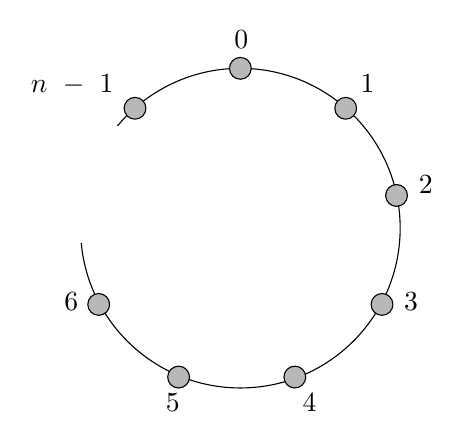
\begin{tikzpicture}[x=0.75pt,y=0.75pt,yscale=-0.7,xscale=0.7]
	%uncomment if require: \path (0,300); %set diagram left start at 0, and has height of 300
	
	%Shape: Circle [id:dp9641223727665371] 
	\draw   (200,150) .. controls (200,89.25) and (249.25,40) .. (310,40) .. controls (370.75,40) and (420,89.25) .. (420,150) .. controls (420,210.75) and (370.75,260) .. (310,260) .. controls (249.25,260) and (200,210.75) .. (200,150) -- cycle ;
	%Shape: Circle [id:dp4867138741225918] 
	\draw  [fill={rgb, 255:red, 184; green, 184; blue, 184 }  ,fill opacity=1 ] (302.5,40) .. controls (302.5,35.86) and (305.86,32.5) .. (310,32.5) .. controls (314.14,32.5) and (317.5,35.86) .. (317.5,40) .. controls (317.5,44.14) and (314.14,47.5) .. (310,47.5) .. controls (305.86,47.5) and (302.5,44.14) .. (302.5,40) -- cycle ;
	%Shape: Circle [id:dp6885524539067742] 
	\draw  [fill={rgb, 255:red, 184; green, 184; blue, 184 }  ,fill opacity=1 ] (375,67.5) .. controls (375,63.36) and (378.36,60) .. (382.5,60) .. controls (386.64,60) and (390,63.36) .. (390,67.5) .. controls (390,71.64) and (386.64,75) .. (382.5,75) .. controls (378.36,75) and (375,71.64) .. (375,67.5) -- cycle ;
	%Shape: Circle [id:dp8052849816078498] 
	\draw  [fill={rgb, 255:red, 184; green, 184; blue, 184 }  ,fill opacity=1 ] (410,127.5) .. controls (410,123.36) and (413.36,120) .. (417.5,120) .. controls (421.64,120) and (425,123.36) .. (425,127.5) .. controls (425,131.64) and (421.64,135) .. (417.5,135) .. controls (413.36,135) and (410,131.64) .. (410,127.5) -- cycle ;
	%Shape: Circle [id:dp7232843669595623] 
	\draw  [fill={rgb, 255:red, 184; green, 184; blue, 184 }  ,fill opacity=1 ] (400,202.5) .. controls (400,198.36) and (403.36,195) .. (407.5,195) .. controls (411.64,195) and (415,198.36) .. (415,202.5) .. controls (415,206.64) and (411.64,210) .. (407.5,210) .. controls (403.36,210) and (400,206.64) .. (400,202.5) -- cycle ;
	%Shape: Circle [id:dp14614821359588803] 
	\draw  [fill={rgb, 255:red, 184; green, 184; blue, 184 }  ,fill opacity=1 ] (340,252.5) .. controls (340,248.36) and (343.36,245) .. (347.5,245) .. controls (351.64,245) and (355,248.36) .. (355,252.5) .. controls (355,256.64) and (351.64,260) .. (347.5,260) .. controls (343.36,260) and (340,256.64) .. (340,252.5) -- cycle ;
	%Shape: Circle [id:dp9823043931092899] 
	\draw  [fill={rgb, 255:red, 184; green, 184; blue, 184 }  ,fill opacity=1 ] (260,252.5) .. controls (260,248.36) and (263.36,245) .. (267.5,245) .. controls (271.64,245) and (275,248.36) .. (275,252.5) .. controls (275,256.64) and (271.64,260) .. (267.5,260) .. controls (263.36,260) and (260,256.64) .. (260,252.5) -- cycle ;
	%Shape: Circle [id:dp9834315290824136] 
	\draw  [fill={rgb, 255:red, 184; green, 184; blue, 184 }  ,fill opacity=1 ] (205,202.5) .. controls (205,198.36) and (208.36,195) .. (212.5,195) .. controls (216.64,195) and (220,198.36) .. (220,202.5) .. controls (220,206.64) and (216.64,210) .. (212.5,210) .. controls (208.36,210) and (205,206.64) .. (205,202.5) -- cycle ;
	%Shape: Rectangle [id:dp07149613177907699] 
	\draw  [draw opacity=0][fill={rgb, 255:red, 255; green, 255; blue, 255 }  ,fill opacity=1 ] (180,80) -- (250,80) -- (250,160) -- (180,160) -- cycle ;
	%Shape: Circle [id:dp5656720700928188] 
	\draw  [fill={rgb, 255:red, 184; green, 184; blue, 184 }  ,fill opacity=1 ] (230,67.5) .. controls (230,63.36) and (233.36,60) .. (237.5,60) .. controls (241.64,60) and (245,63.36) .. (245,67.5) .. controls (245,71.64) and (241.64,75) .. (237.5,75) .. controls (233.36,75) and (230,71.64) .. (230,67.5) -- cycle ;
	
	% Text Node
	\draw (195.37,127.24) node [anchor=north west][inner sep=0.75pt]  [rotate=-289.59]  {$\dotsc $};
	% Text Node
	\draw (304,12.4) node [anchor=north west][inner sep=0.75pt]    {$0$};
	% Text Node
	\draw (391,42.4) node [anchor=north west][inner sep=0.75pt]    {$1$};
	% Text Node
	\draw (431,112.4) node [anchor=north west][inner sep=0.75pt]    {$2$};
	% Text Node
	\draw (421,192.4) node [anchor=north west][inner sep=0.75pt]    {$3$};
	% Text Node
	\draw (351,262.4) node [anchor=north west][inner sep=0.75pt]    {$4$};
	% Text Node
	\draw (257,262.4) node [anchor=north west][inner sep=0.75pt]    {$5$};
	% Text Node
	\draw (187,192.4) node [anchor=north west][inner sep=0.75pt]    {$6$};
	% Text Node
	\draw (164,42.4) node [anchor=north west][inner sep=0.75pt]    {$n\ -\ 1$};
	
	
	\end{tikzpicture}
\end{center}
With this mental picture, we can begin to build up some properties of modular arithmetic.

\begin{proposition}[Arithmetic Modulo $n$]
	If $a \equiv a' \pmod{n}$ and $b \equiv b' \pmod{n}$, then $a + b \equiv a' + b' \pmod{n}$ and $ab \equiv a'b' \pmod{n}$.
\end{proposition}
\begin{proof}
	We have $a' = a + kn$ and $b' = b + jn$, for some $k, j \in \Z$.
	So $a' + b' = a + b + (k + j)n \equiv a + b \pmod{n}$, and $a'b' = (a + kn)(b + jn) = ab + (bk + aj + kjn)n\equiv ab \pmod{n}$.
\end{proof}

Many of the other rules of arithmetic are inherited from $\Z$, for example we have $a + b \equiv b+a \pmod{n}$ as $a + b = b + a$ in $\Z$. Also some of the number-theoretic facts we have previously established can be expressed in modular arithmetic.

\begin{example}[Euclid's Lemma in Modular Arithmetic]
	The statement that for a prime $p$, `$p \mid ab \implies p \mid a$ or $p \mid b$' is equivalent saying that $ab \equiv 0 \pmod{p}$ implies that $a \equiv 0 \pmod{p}$ or $b \equiv 0 \pmod{0}$.
\end{example}

\subsection{Modular Inverses}

We will now begin to look at the multiplicative structure of $\Z/n\Z$. 

\begin{definition}[Modular Inverses]
	For $a, b \in \Z$, we say that $b$ is an \vocab{inverse} of $a$ if $ab \equiv 1 \pmod{n}$.\footnote{This should be reminiscent of the notion of inverses from group theory.}
\end{definition}

\begin{example}
	In $\Z/10\Z$, the inverse of $3$ is $7$, as $3\times 7 = 21\equiv 1 \pmod{10}$. The inverse of $4$ does not exist, as for all $x \in \Z$, $4x \not\equiv 1 \pmod{10}$, as $4x$ is even.

	This example shows that inverses do not always exist for an arbitrary modulus $n$.
\end{example}

\begin{notation}
	We write $a^{-1}$ to mean the inverse of $a$ (modulo some $n$).
\end{notation}

\begin{proposition}[Properties of Modular Inverses]
	In $\Z/n\Z$,
	\begin{enumerate}[label=(\roman*)]
		\item If a modular inverse exists, then it is unique modulo $n$.
		\item If $a$ has an inverse, and $ab \equiv ac \pmod{n}$, then $b \equiv c \pmod{n}$. That is, we can cancel invertible elements.\footnote{We \emph{cannot} cancel elements in general.}
	\end{enumerate}
\end{proposition}
\begin{proof}
	To show (i),
	suppose there exists $b, c \in \Z$ such that for some $a$, $ab \equiv ac \equiv n \pmod{n}$. Then $b(ac) \equiv bab \implies c \equiv b \pmod{n}$. Then to show (ii), we can just multiply both sides by $a^{-1}$.
\end{proof}

When we are working modulo a prime, things tend to be `nicer'.

\begin{proposition}
	Let $p$ be a prime, then every $a \neq 0 \pmod{p}$ has an inverse modulo $p$.
\end{proposition}
\begin{proof}
	We have $\gcd(a, p) = 1$, so we can write $ax + py = 1$ for some $x,y \in \Z$. But then $ax = 1 - py$, and thus $ax \equiv 1 \pmod{p}$.\hfill\qed

	\emph{Alternate Proof}. 
	In $\Z/n\Z$, consider the multiplies of a: $0\times a$, $1 \times a$, $2 
	\times a$, $\dots$, $(p - 1)\times a$. We wish to show that one of them is $1$. We have $p$ items written down, and I claim these are all \emph{distinct} in $\Z/p\Z$. If $ia = ja \implies (i - j)a \equiv 0$, which implies $a \equiv 0$ or $i -j \equiv 0 \implies i \equiv j \pmod{p}$. Hence, there must be $0$, $1$, $\dots$, $p - 1$ in this list, in some order. Thus $xa \equiv 1 \pmod{p}$, for some $x \in \Z/n\Z$.
\end{proof}

We can generalize this proposition by considering which properties of the primes we used in the previous proof.

\begin{proposition}
	Let $n \in \N$. Then $a$ has an inverse modulo $n$ if and only if $\gcd(a, n) = 1$.
\end{proposition}
\begin{proof}
	We have $\gcd(a, n) = 1 \iff ax + ny = 1$, for some $x, y \in \Z$. Then $ax = 1 - ny \equiv 1 \pmod{n}$.
\end{proof}

There is a commonly used function to count how many elements have an inverse modulo some $n$.

\begin{definition}[Euler's Totient Function]
	Euler's totient function $\phi(n)$ is the number of numbers $1, 2, \dots, n$ that are relatively prime to $n$.
	This function counts the number of invertibles or \vocab{units} in $\Z/n\Z$.
\end{definition}

\begin{example}
	If $p$ is a prime, then $\phi(p) = p - 1$, $\phi(p^2) = p^2 - p$ (we cannot have $p, 2p, \dots, pp$). If $p$ and $q$ are distinct primes, then $\phi(pq) = pq - p - q + 1$.
\end{example}

\subsection{Exponentiation}

Consider the powers of 2 in $\Z/7\Z$. We have the sequence
\begin{align*}
	2^1 &\equiv 2 \pmod{7}\\
	2^2 &\equiv 4 \pmod{7}\\
	2^3 &\equiv 1 \pmod{7}\\
	2^4 &\equiv 2 \pmod{7}\\
		&\vdots
\end{align*}
This sequence will repeat periodically, with a period of 3.
It turns out that in general, this will always occur. This can be seen in the following theorem, which turns out to be an incredibly important result which is used all the time. This theorem has many proofs, but we present one particularity nice one, which emphasizes the theory that we have developed so far.

\begin{theorem}[Fermat's Little Theorem]
	Let $p$ be a prime, then for $a \not\equiv 0 \pmod{p}$, we have 
	$$a^{p - 1} \equiv 1 \pmod{p}.$$
\end{theorem}
\begin{proof}
	Consider the numbers $1 \cdot a$, $2 \cdot a$, $\dots$, $(p - 1) \cdot a$ modulo $p$. They are distinct, as if $a i \equiv aj$ then $i \equiv j \pmod{p}$, because $a$ is invertible. They are also non-zero. So we must have the numbers $1, 2, \dots, p - 1 \pmod{p}$ in some order. Then, if we multiply together we have
	$$
	a^{p - 1} (p - 1)! \equiv (p - 1)! \pmod{p},
	$$
	so we can cancel $(p - 1)!$ as it's the product of invertibles, to obtain $a^{p - 1} \equiv 1 \pmod{p}$.
\end{proof}

As before, we can consider what happens in the case of a non-prime modulus.

\begin{theorem}[Fermat-Euler Theorem]
	Let $n \in \N$. Then for $a \not \equiv 0 \pmod{n}$, we have
	$$
	a^{\phi(n)} \equiv 1 \pmod{n}.
	$$
\end{theorem}
\begin{proof}
	We copy the proof of Fermat's little theorem. Let the units in $\Z/n\Z$ be $x_1, \dots, x_{\phi(n)}$. Consider $a \cdot x_1$, $a \cdot x_2$, $\dots$, $a \cdot x_{\phi(n)}$. They are distinct and invertible as before, so they must be $x_1, \dots, x_{\phi(n)}$ in some order. Multiplying them all together,
	$$
	a^{\phi(n)} x_1 x_2 \cdots x_{\phi(n)} \equiv x_1 x_2 \cdots x_{\phi(n)} \pmod{n},
	$$
	and then we can cancel each $x_i$ to obtain $a^{\phi(n)} \equiv 1 \pmod{n}$.
\end{proof}

We can pause for a moment and notice that in the proof of Fermat's little theorem, we could cancel $(p - 1)! \pmod{p}$ because it was non-zero. So what exactly was it? We can try an example of $p = 5$, then we have $4! = 1 \equiv 24 \equiv - 1 \pmod{5}$. We can also try $p = 7$ to get $6! = 720 \equiv -1 \pmod{7}$. It can be proved that this is always the case.

First, we prove a small lemma.

\begin{lemma}\label{lemma:root-1-mod-p}
	Let $p$ be prime, then $x^2 \equiv 1 \pmod{p}$ implies $x \equiv 1$ or $x \equiv -1 \pmod{p}$.\footnote{Note that this is only true because $p$ is prime. For example, $1^2 \equiv 3^2 \equiv 5^2 \equiv 7^2 \equiv 1 \pmod{8}$.}
\end{lemma}
\begin{proof}
	$x^2 \equiv 1 \implies x^2 - 1 \equiv 0 \pmod{p}$, which we can factor as $(x + 1)(x - 1) \equiv 0 \pmod{p}$ and thus $x \equiv 1$ or $x \equiv -1 \pmod{p}$.
\end{proof}
\begin{remark}
	It turns out that for a prime $p$, a non-zero polynomial in $\Z/p\Z$ of degree $k$ always has at most $k$ roots.
\end{remark}

We can now prove our result about the value of $(p - 1)! \pmod{p}$.

\begin{theorem}[Wilson's Theorem]
	Let $p$ be a prime, then
	$$
	(p - 1)! \equiv - 1\pmod{p}.
	$$
\end{theorem}
\begin{proof}
	Note that this is true for $p = 2$, so we may assume that $p \geq 2$. Consider the numbers $1, 2, \dots, p - 1$ modulo $p$. We can pair up each $a$ with its inverse $a^{-1}$ for $a \neq a^{-1}$. But $a = a^{-1} \iff a^2 = 1$, so the only elements that are their own inverse are $1$ and $-1$. Thus $1, 2, \dots, p - 1$ consists of some pairs $a, a^{-1}$ and $1$ and $-1$. Thus when we multiply,
	$
	(p - 1)! \equiv 1^{\frac{p - 3}{2}} \cdot 1 \cdot -1 \equiv -1 \pmod{p}.
	$
\end{proof}

To see how we can use both Wilson's theorem and Fermat's little theorem together, we can consider another question that follows naturally from \autoref{lemma:root-1-mod-p}.

\begin{lemma}[$x^2 + 1$ Lemma]
	Let $p$ be an odd prime. Then $x^2 \equiv -1 \pmod{-1}$ has a solution if and only if $p \equiv 1 \pmod{4}$.
\end{lemma}
\begin{proof}
	If $p = 4k + 3$, suppose that $x^2 \equiv -1 \pmod{p}$. Then we have from Fermat's little theorem that $x^{4k + 2} \equiv 1 \pmod{p}$, but $x^{4k + 2} \equiv (x^2)^{2k + 1} \equiv (-1)^{2k + 1} \equiv -1$, which is a contradiction.

	We now construct an example to show that $p \equiv 1 \pmod{4}$ works. By Wilson's theorem, $(4k!) \equiv -1 \pmod{p}$. Then, noting that $4k - j \equiv -j - 1 \pmod{p}$, $(2k)!^2 \equiv (2k!)^2 \cdot (-1)^{2k} \equiv (4k)! \equiv -1 \pmod{p}$, so a solution exists.
\end{proof}

\subsection{Congruence Equations and the Chinese Remainder Theorem}

We now return back to the topic of linear diophantine equations, this time looking specifically at linear congruence equations. Let's look at an example. 

\begin{example}[Solving a Linear Congruence Equation]
	Solve $7x \equiv 4 \pmod{30}$.
\end{example}
\begin{proof}[Solution]
	First we \emph{find a solution}.

	We have $\gcd(7, 30) = 1$, so we can run the Euclidean algorithm on $7$ and $30$ to obtain $7 \times 13 - 30 \times 3 = 1$. So $7 \times 13 \equiv 1 \pmod{30}$, hence $7 \times 52 \equiv 4 \pmod{30}$. So $x \equiv 52 \pmod{30}$ is a solution.

	Now we show there is \emph{no more solutions}.

	If $x'$ is a solution, then we have $7x \equiv 4 \pmod{30}$ and $7x' \equiv 4 \pmod{30}$. Thus $7x \equiv 7x' \pmod{30}$, which implies that $x \equiv x' \pmod{30}$ as $7$ is invertible.
	So $x \equiv 52 \pmod{30}$ is the only solution.
\end{proof}

There is a shorter method that can be used too, if we can quickly spot the inverse of the coefficient of our variable.

\begin{example}
	Solve $3x \equiv 9 \pmod{28}$.
\end{example}
\begin{proof}[Solution]
	$3x \equiv 9 \pmod{28} \iff 19 \cdot 3 x \equiv 19 \cdot 9 \pmod{28}$, as $19$ is invertible. Thus $x \equiv 171 \equiv 3 \pmod{8}$.
\end{proof}

If we don't have that the coefficient and the modulus is coprime, it's typically easier to write the equation as a standard linear diophantine equation.

\begin{example}
	Solve $10x \equiv 12 \pmod{34}$.
\end{example}
\begin{proof}[Solution]
	$10x \equiv 12 \pmod{34} \iff 10x = 12 + 34 y$ for some $y \in \Z$. Then $10x = 12 + 34y \iff 5x = 6 + 17 y$, which we can write as $5x \equiv 6 \pmod{17}$. We can then solve as before. 
\end{proof}

Now consider a simultaneous congruence equation. Specifically, consider the equations
\begin{align*}
	x &\equiv 6 \pmod{17} \\
	x &\equiv 2 \pmod{19}.
\end{align*}
Do we expect a solution to this? We might guess yes, as $17$ and $19$ are coprime, so intuitively `modulo 17 and modulo 19 should be independent of each other'. What about these equations:
\begin{align*}
	x &\equiv 6 \pmod{34} \\
	x &\equiv 11 \pmod{36}.
\end{align*}
We shouldn't expect solutions to these equations. Even if you try and figure out if $x$ is even or odd, you'll run into issues. This intuition can be formalized into a theorem.

\begin{theorem}[Chinese Remainder Theorem]
	Let $m$ and $n$ be relatively prime positive integers. Then for any integers $a$ and $b$, there is solution to
	\begin{align*}
		x &\equiv a \mod{m} \\
		x &\equiv b \mod{n},
	\end{align*}
	and this solution is unique modulo $mn$. 
\end{theorem}
\begin{proof}
	First we prove existence. We have $ms + nt = 1$ for some $s, t \in \Z$ by Bezout's lemma. Then $ms \equiv 0 \mod{m}$ and $1 \pmod{n}$ and $nt \equiv 0 \pmod{n}$ and $1 \pmod{m}$. Hence
	$x = a(nt) + b(ms)$ has $x \equiv a \pmod{m}$ and $x \equiv b \pmod{n}$.

	To show uniqueness, certainly any $x' \equiv x \pmod{mn}$ is also a solution. Conversely, suppose $x'$ has $x' \equiv a \pmod{m}$ and $b \pmod{n}$. Then $x' \equiv x \pmod{m}$ and $x' \equiv x \pmod{n}$, that is, $m \mid x' - x$ and $n \mid x' - x$. Thus $mn \mid x' - x$, as $\gcd(m, n) = 1$, and thus $x' \equiv x \pmod{mn}$.
\end{proof}

This theorem generalizes directly.

\begin{theorem}[General Chinese Remainder Theorem]
	Let $m_1$, $\dots$, $m_k$ be pairwise relatively prime positive integers, and let 
	$$M = m_1 m_2 \cdots m_k.
	$$ Then for all integers $x_1, \dots, x_k$, the equations
	\begin{align*}
		x & \equiv x_1 \pmod{m_1} \\
		x & \equiv x_2 \pmod{m_2} \\
			& \;\vdots \\
		x & \equiv x_k \pmod{m_k}
	\end{align*}
	have a solution $x$ that is unique modulo $M$.
\end{theorem}
\begin{proof}[Proof Sketch]
	Reduce the number of equations by applying the two variable Chinese remainder theorem to the last two equations.
\end{proof}

\subsection{An Application of the Fermat-Euler Theorem: RSA Encryption}

RSA is an algorithm that underpins a huge amount of modern cryptography and security. 

Normally, to send a coded message to someone, you would encode the message, which you could then send to the intended receiver who would decode it. This decoding would be performing the encoding operation in reverse -- they are inverse operations. Because of this, it would seem obvious in this way that knowing how to encode is the same as knowing how to decode.
For example, if your encoding is `add 1 to each letter', a \emph{
	Caesar cipher}, then you immediately know how to decode: `take 1 from each letter'.
	For another example, if your encoding is `add 1 to each letter then reverse each word', then to decode you `reverse each word and subtract 1 to each letter'. 
This belief, that knowing how to encrypt implies knowing how to decrypt, was held for centuries, but it isn't quite correct. We will see this in the RSA encryption system.

Begin with two large distinct primes $p$ and $q$, and let $n = pq$. Let's say we want to encrypt some element $x \in \Z/n\Z$ -- this may involve taking the message we want to send and splitting it up in some way. We will do that in the following way.

Fix a `coding exponent' $e$.
To encode a message $x \in \Z/n\Z$, raise it to the power $e$.
$$
x \longmapsto x^e.
$$

Now let's figure out how to decode this message. We want some $d \in \Z/n\Z$ so that $(x^e)^d \equiv x \pmod{n}$. First, assume that $x$ and $n$ are coprime (ensure that the message $x$ is constructed to have this condition).
We know from the Fermat-Euler theorem that $x^{\phi(n)} \equiv 1 \pmod{n}$, and also that $x^{k \phi(n)} \equiv 1 \pmod{n}$, for all $k \in \Z$. So we have
$$
x^{k \phi(n) + 1} \equiv x \pmod{n}.
$$
So it suffices to find a $d$ such that $de = k \phi(n) + 1$, for some $k \in \Z$. That is, we want an inverse of $e$ modulo $\phi(n)$. We can do this by running the Euclidean algorithm on the numbers $e$ and $\phi(n)$. This implies we needed to have picked $e$ coprime with $\phi(n)$.

With the encryption and decryption methods defined, we can now consider what information is needed to perform each step.

To encode, we take $x \longmapsto x^e \pmod{n}$\footnote{This process can be done quite quickly by squaring the number whenever possible.}. This means we need to know that will need to know $n$ (so you know what modulus to use) and also the power $e$.

To decode, we take $y \longmapsto y^d \pmod{n}$, so we need to know $n$ and $d$. But we worked out $d$ as the inverse of $e$ modulo $\phi(n)$, so we really need $n$, $e$ and $\phi(n)$. Recall that
$$
\phi(n) = n - p - q + 1.
$$
So to compute $\phi(n)$, we need to know the factors of $n$.
However, the problem of factoring $n$ is thought to be incredibly hard, and the best known methods of today would take longer than the age of the universe to factor $n$ into two $100$ digit long primes. 
This means that if $e$ and $n$ were published, then anyone could encode a message, but only you (or someone who knows the factors of $n$) would be able to decode. So, with RSA encryption, anyone can encrypt a message and send it to you, but only you can decrypt it.


\chapter{The Reals}

Moving on from number theory, this chapter will center on the questions of \emph{what is a real number} and \emph{what can we assume like them}.
Unlike when we defined the natural numbers, in this chapter we will not just define the reals formally and then proceed as normal; instead, we will try and understand some of the more subtle aspects of the real numbers, that will eventually be carried through in `Analysis'.

\section{Why We Need Real Numbers}

Recall that in \autoref{ch:1}, we began by defining the natural numbers $\N$, extended them to the integers $\Z$, and extended them to the rationals $\Q$. So why would we not stop there? In the following example, we will show that for some (many) purposes, the rationals are not adequate.

\begin{proposition}
	There is no $x \in \Q$ such that $x^2 = 2$.
\end{proposition}
\begin{proof}
	Assume that $x \geq 0$. If there was such a rational, we could write
	$$
	x = \frac{a}{b},
	$$
	where $a, b \in \Z$. We can square this to get
	$$
	x^2 = \frac{a^2}{b^2} = 2 \implies a^2 = 2b^2,
	$$
	but this is a contradiction of the fundamental theorem of arithmetic, as the power of 2 in $a^2$ would have to be odd\footnote{The same proof shows that if there exists $x \in \Q$ so that $x^2 = n$, for $n \in \N$, then $n$ must be a square number. This is because each exponent in the prime factorisation of $n$ must be even.}.\hfill\qedhere

	\emph{Alternate Proof}. Suppose that for some $x = a/b \in \Q$ where $a, b \in \N$, we have $x^2 = 2$. Note that for any integers $c$ and $d$, the number $cx + d$ is of the form $e/b$, for some $e \in \Z$. So, if $cx + d > 0$, then $cd + d > \frac{1}{b}$. But $x^2 = 2 \implies 0 < x - 1 < 1$, we can say $0 < (x - 1)^k < 1/b$ for large enough $k$. But this is a contradiction, because $(x - 1)^k$ is of the form $cx + d$.\hfill\qed
\end{proof}

Informally, what this result shows is that $\Q$ has a `gap' at $\sqrt{2}$, and in constructing the reals, we will try formally define a number system that has no such `gaps'. This immediately raises the question of how we can define such a system, formalizing our rather vague notion of a `gap'. This must be done while only making statements about the rationals.  


Consider again our example that there is no rational $x$ such that $x^2 = 2$. With this in mind, define the set $S$ as follows:
$$
S = \{ x \in \Q \; : \; x^2 < 2\}.
$$
We will now think about bounds on the elements in this set.

\begin{definition}
	A set $S$ is \vocab{bounded above} if there exists $x \in \R$ with $x \geq y$ for all $y \in S$. Such an $x$ is a \vocab{least upper bound} of $S$ if $x$ is an upper bound for $S$, and every upper bound $x'$ of $S$ satisfies $x < x'$. 
\end{definition}

It should be clear that $1.5$ is an upper bound on the elements in this set. $1.42$ is also an upper bound. By setting such upper bounds, we can get arbitrarily close to a number $x$ such that $x^2 = 1$, that is there cannot be a \emph{least} upper bound. If there was, it would have to be a number so that $x^2 = 2$, but we know there isn't such a rational. 
It's using this idea of `least upper bounds' that we can define the reals.

\begin{definition}[The Reals]
	The \vocab{reals} are a set $\R$ with elements $0$ and $1$ (where $0 \neq 1$), along with operations $+$ and $\times$ and an ordering $<$ such that:
	\begin{enumerate}
		\item $+$ is commutative, associative, has an identity $0$, and every $x \in \R$ has an inverse.
		\item $\times$ is commutative, associative, has an identity $1$, and every $x \in \R$ where $x \neq 0$ has an inverse.
		\item $\times$ is distributive over $+$.
		\item $\forall a, b$, exactly one of $a < b$, $a = b$ and $b < a$ holds. Also if $a < b$ and $b < c \implies a < c$.
		\item $\forall a, b, c \in \R$, $a < b \implies a + c < b + c$ and $a < b \implies ac < bc$ if $c > 0$.
		\item \emph{Least Upper Bound}. Every non-empty set of reals that is bounded above has a least upper bound.
	\end{enumerate}
\end{definition}

It's worth noting that the conditions in axiom 6 of the set of reals being `non-empty' and `bounded above' is needed because if there was no upper bound, then there is certainty no \emph{least} one. Also, if the set was empty then every $x \in \R$ would be an upper bound, and there would be no least one.

From these axioms, it's straightforward to check some very basic facts, for example that $0 < 1$.
\begin{example}
	We have $0 < 1$.
\end{example}
\begin{proof}
	If that were not the case, as we have $0 \neq 1$ as an axiom, we would need $1 < 0$. 
	This would imply $0 < -1$ and thus it is `positive', 
	so we can multiply by the `positive' -1 to get $0 < 1$, which contradicts our assumption.
\end{proof}

We can also (as you may expect) view $\mathbb{Q}$ as contained in $\mathbb{R}$, by identifying $a/b \in \Q$ with $a, b^{-1} \in \R$. In this system, axioms 1 to 5 hold, but axiom 6 does not hold.
We have defined the reals here by specifying the axioms that they satisfy, but that is not the only way. It is possible to construct $\R$ from $\Q$, in a way that is (vaguely) similar to the way we constructed $\Q$ from $\Z$. This is, surprisingly, not as helpful as one might imagine, so we will skip over this topic for now.

\subsection{Least Upper Bounds}

The notion of least upper bounds is so central to the real numbers that we will consider some examples of different sets and their least upper bounds, in order for you to get see some of the properties. We will use the following notation for the least upper bound.

\begin{definition}[Supremum]
	The least upper bound of a set $S$ is also known as the \vocab{supremum} of $S$, written $\sup S$.
\end{definition}

\begin{example}[Sets and Least Upper Bounds]~
    \vspace*{-\baselineskip}
\begin{enumerate}
	\item The set $S = \{x \in \R : 0 \leq x \leq 1\}$ has a least upper bound $x = 1$. This is because $1$ is an upper bound, and also every upper bound $y$ has $y \geq 1$, as $1 \in S$.
	\item Consider the set $S = \{ x \in \R : 0 < x < 1\}$. We have $2$ as an upper bound, as $x \in S$ has $x < 1 < 2$. Also $3/4$ is not an upper bound, as $7/8 \in S$, and $3/4 < 7/8$. Now the least upper bound of $S$ is $1$, because $1$ is an upper bound, and no upper bound $c$ has $c < 1$, as otherwise, $c \in S$, and we can take $c + (1 - c)/2 \in S$.
	\item $S = \left\{1 - \frac{1}{n}  : n \in \N \right\} = \left\{0, \frac{1}{2}, \frac{2}{3}, \frac{3}{4}, \dots \right\}$. Clearly $1$ is an upper bound, and we will return to this example to show that it is the least upper bound.
\end{enumerate}
\end{example}

\begin{theorem}[Axiom of Archimedes]
	$\mathbb{N}$ is not bounded above in $\R$.
\end{theorem}
\begin{proof}
	Let's suppose that it was bounded above, in which case we would have $c = \sup \N$, for some $c \in \R$. So $c - 1$ is \emph{not} an upper bound for $\N$. That implies that there is a natural number $n$ with $n > c - 1$. But then $n +1 \in \N$, and $n + 1 > c$, which is a contradiction.
\end{proof}

\begin{corollary}
	For each $t > 0$, there exists $n \in \N$ with $\frac{1}{n} < t$.
\end{corollary}
\begin{proof}
	We have some $n \in \N$ with $n > \frac{1}{t}$ by the previous result, so $\frac{1}{n} < t$.
\end{proof}

\begin{remark}
	Informally, these two results are telling us that $\R$ does not contain any `infinitely big' or `infinitesimally small' elements.
\end{remark}

We can return to the third example above, and we can now show that $\sup S = 1$, as if there was some $c < 1$ that was an upper bound, then $1 - \frac{1}{n} < c$ for every $n \in \N$, so $1 - c < \frac{1}{n}$, which is impossible (by the corollary we just proved).

\begin{remark}[Warning]
	If a set $S$ has a greatest element (like $[0, 1]$), then that greatest element is $\sup S$, so $\sup S \in \S$. But if $S$ has no greatest element (like $(0, 1)$), then $\sup S \not\in S$.
\end{remark}

We have been discussing upper bounds of sets, but the least upper bound axiom also implies some facts about lower bounds.

\begin{definition}
	A set $S$ is \vocab{bounded below} if there exists $x \in \R$ with $x \leq y$ for all $y \in S$. Such an $x$ is a \vocab{greatest lower bound} of $S$ if $x$ is a lower bound for $S$, and every lower bound $x' \neq x$ of $S$ satisfies $x < x'$.
	We write $x = \inf S$.
\end{definition}

\begin{proposition}
If a set $S$ is non-empty and has a lower bound, then it has a greatest lower bound.	
\end{proposition}
\begin{proof}
	Let the set $-S = \{-y : y \in S\}$. It is non-empty and bounded above, so it has a least upper bound $c$. So $-c$ is the greatest lower bound of $S$, $\inf S$.
\end{proof}

\subsection{Rationals and Irrationals}

Let's return to our original question which prompted our discussion of the real numbers: that there is no $x \in \Q$ with $x^2 = 2$. If we have in any way succeeded, we should be able to do somewhat better than that in the reals. 

\begin{proposition}
	There is some $x \in \R$ such that $x^2 = 2$.
\end{proposition}
\begin{proof}
	Let $S = \{x \in \R, x^2 < 2\}$. We have $S$ is nonempty, and it is bounded above, so $c = \sup S$ for some $c \in \R$. We claim that $c^2 = 2$. If this wasn't the case, then either $c^2 < 2$ or $c^2 > 2$. If $c^2 < 2$, then for $t < \frac{2 - c^2}{4}$ we have $(c + t)^2 < 2$, which contradicts $c$ being an upper bound for $S$. If $c^2 > 2$, then we can let $t < \frac{c^2 - 2}{4}$ and then $(c - t)^2 > 2$, which contradicts that $c$ is the \emph{least} upper bound for $S$. So we must have $c^2 = 2$.
\end{proof}

This same proof also shows that $\sqrt[n]{x}$ exists for all $n \in \N$ and $x \in \R$. 
We regularly distinguish between a real number that is also a rational number, and a real number that is not also a rational.

\begin{definition}
	A real that is not rational is called an \vocab{irrational}.
\end{definition}


\begin{example}
	$\sqrt{2}$, $\sqrt{3}$, $\sqrt{6}$ and $\sqrt{15}$ are all irrational, as is $2 + 3\sqrt{5}$.
\end{example}

It's worth noting that the rationals are \vocab{dense} in the reals.

\begin{theorem}[$\Q$ is dense in $\R$]
		The rationals are \vocab{dense} in $\R$, that is, for $a, b \in \R$, there exists $q \in \Q$ such that $a \leq q \leq b$.
\end{theorem}
\begin{proof}
	Without loss of generality, assume that $a, b \geq 0$. Then choose some $n \in \N$ such that $\frac{1}{n} < b - a$. Then among
	$\frac{0}{n}, \frac{1}{n}, \dots$, there is a \emph{final} one that is less than or equal to $a$, say $\frac{k}{n}$. So $a < \frac{q + 1}{n} < b$.
\end{proof}

Slightly more interesting is the following result.
\begin{theorem}
	The irrationals are dense, that is, for $a, b\in\R$ with $a<b$, there exists an irrational $c$ such that $a < c < b$.
\end{theorem}
\begin{proof}
	This follows from the rational case, as we can find a rational $c$ between $\sqrt{2}a$ and $\sqrt{2}b$, then $c/\sqrt{2}$ is irrational, and lies between $a$ and $b$.
\end{proof}

\section{Sequences}

We are now going to discuss one of the major uses of the least upper bound statement -- sequences. We are going to consider some questions like
$$
\text{What should } 1 + \frac{1}{2} + \frac{1}{4} + \cdots = 2 \text{ mean?}
$$
and 
$$
\text{What should } 0.3333\dots = \frac{1}{3} \text{ mean?}
$$

For the first question, presumably the first sequence should `tend to' 2, and the second should `tend to' $1/3$. So what does it mean for a sequence $x_1$, $x_2$, $\dots$ to `tend to' some $c$? It should not mean that $x_n$ is getting closer to $c$, for example, we would not want $1/2$, $2/3$, $3/4$, $\dots$ to tend to 17. We also don't mean that $x_n$ gets arbitrarily close to $c$, as for example, the sequence $1/2$, $10$, $2/3$, $10$, $\dots$ should not tend to 1.
The correct way to think of it is that we will get arbitrarily close \emph{and stay} within some value of $c$.

\begin{definition}
	We say that a sequence of reals $x_1$, $x_2$, $\dots$ \vocab{tends to} $c \in \R$ if $\forall \varepsilon > 0$, there exists $n \in \N$ such that
	$$
	|x_n - c| < \epsilon.
	$$
\end{definition}

\begin{remark}[Informal]
	We can think of this say saying `$\forall \varepsilon > 0$, $x_n$ eventually is within $\varepsilon$ of $c$'.
\end{remark}

There is quite a lot of subtlety to this definition, so we will spend some time considering it's consequences.

\begin{notation}
	If $x_n$ tends to $c$, we will write $x_n \rightarrow c$, or $x_n \rightarrow c$ as $n \rightarrow \infty$, or $\lim_{n \to \infty} x_n = c$.
\end{notation}

% \begin{center}
	

% \tikzset{every picture/.style={line width=0.75pt}} %set default line width to 0.75pt        

% \begin{tikzpicture}[x=0.75pt,y=0.75pt,yscale=-1,xscale=1]
% %uncomment if require: \path (0,300); %set diagram left start at 0, and has height of 300

% %Straight Lines [id:da9270971168871558] 
% \draw    (113,150) -- (507,150) ;
% \draw [shift={(510,150)}, rotate = 180] [fill={rgb, 255:red, 0; green, 0; blue, 0 }  ][line width=0.08]  [draw opacity=0] (8.93,-4.29) -- (0,0) -- (8.93,4.29) -- cycle    ;
% \draw [shift={(110,150)}, rotate = 0] [fill={rgb, 255:red, 0; green, 0; blue, 0 }  ][line width=0.08]  [draw opacity=0] (8.93,-4.29) -- (0,0) -- (8.93,4.29) -- cycle    ;
% %Straight Lines [id:da7047009712473145] 
% \draw    (210,150) -- (210,160) ;
% %Straight Lines [id:da8253037934553922] 
% \draw    (310,150) -- (310,160) ;
% %Straight Lines [id:da10189023146303988] 
% \draw    (360,150) -- (360,160) ;
% %Straight Lines [id:da7264863609117935] 
% \draw    (260,150) -- (260,160) ;
% %Straight Lines [id:da3399652653596268] 
% \draw    (160,150) -- (160,160) ;
% %Straight Lines [id:da011826230856242015] 
% \draw    (410,150) -- (410,160) ;
% %Straight Lines [id:da07377146344311347] 
% \draw    (460,150) -- (460,160) ;

% % Text Node
% \draw (148,162.4) node [anchor=north west][inner sep=0.75pt]    {$-2$};
% % Text Node
% \draw (198,162.4) node [anchor=north west][inner sep=0.75pt]    {$-1$};
% % Text Node
% \draw (254,162.4) node [anchor=north west][inner sep=0.75pt]    {$0$};
% % Text Node
% \draw (304,162.4) node [anchor=north west][inner sep=0.75pt]    {$1$};
% % Text Node
% \draw (354,162.4) node [anchor=north west][inner sep=0.75pt]    {$2$};
% % Text Node
% \draw (404,162.4) node [anchor=north west][inner sep=0.75pt]    {$3$};
% % Text Node
% \draw (454,162.4) node [anchor=north west][inner sep=0.75pt]    {$4$};


% \end{tikzpicture}
% \end{center}



% \chapter{Sets and Functions}

% \chapter{Countability}







\clearpage
\chapter*{Bibliography}

\begin{itemize}
	\item T. Tao, \emph{Analysis I}
	
	This book provides discussion of the Peano axioms, along with some relevant proofs that were (purposefully) excluded from the lectures. The treatment of the Peano axioms in these notes follow this exposition closely.
\end{itemize}

% TODO: Make this proper.

% \begin{itemize}
% 	\item Napkin by Evan Chen -- Used for a good few of the examples
% 	\item Abstract Algebra by Dummit and Foote -- General Reference
% 	\item A Book of Abstract Algebra, Charles Pinter -- General Reference
% 	\item Dexter Chua and David Bai's notes -- For a general view on the course structure before the lectures were completed, along with some of the proofs that were omitted from our lectures.
% \end{itemize}

% \begin{itemize}
% 	\item Analysis I by Terry Tao -- Used for discussion about defining the natural numbers, along with examples and proofs that were excluded in lectures.
% \end{itemize}

% \nocite{*}
% \printbibliography

\end{document}
